Most hierarchical clustering algorithms
produce a binary tree over the data,
where each leaf corresponds to a data point.
Internal nodes correspond to groupings of descendant leaves.
This approach is simple, but can run into
problems when the hierarchical structure
in the data is ambiguous. Consider
a simple dataset with three points
that are equidistant from each other 
or a dataset with three points
lying equally spaced apart in a line (see \autoref{fig:ambiguous-structure}).
A single binary tree is not sufficient
to describe the similarity relationships
between the points, as a single tree
will imply that some points are more similar
to each other than the other
when they are in fact not.
An initial solution is to extend clustering
algorithms to produce trees with arbitrary
branching factors.
This will help solve the
ambiguity problem
in the first dataset, but
not the second.
Furthermore, we can construct 
adversarial datasets
that will always be ambiguous.
Consider $\numdata$ points lying on the unit circle, equally spaced apart.
Due to rotational symmetry, there will be several
equivalent trees with max branching factor less than $\numdata$.
Since an $\numdata$-ary tree over $\numdata$ data points
implies no underlying structure,
we require an approach that can
handle ambiguity without compromising
the capacity to discover structure.

Bayesian nonparametric hierarchical clustering (BNHC)
addresses the general issue of
ambiguity in hierarchical structure
by explicitly modeling any uncertainty with probability.
Rather than outputting a single tree
as in traditional hierarchical clustering,
a Bayesian method
returns a probability distribution
over hierarchies that explain the data.
In the ambiguous dataset with three points described earlier,
a Bayesian method would return
a distribution over the three hierarchies,
where each is assigned
a probability of $1/3$.
BNHC
also follows the standard Bayesian paradigm,
where Bayes rule enables
calculating a posterior distribution
given a prior and a likelihood model.

%The chapter is organized as follows.
%In section 2 we provide background information
%about traditional hierarchical clustering
%methods and Bayesian learning.
%In section 3 we lay down the fundamentals
%of Bayesian hierarchical clustering,
%describe several of the prominent
%models in BNHC, and provide
%algorithms to perform inference in the models.
%In section 4 we introduce ideas
%to improve BNHC with user interaction,
%and in section 5, we conclude and describe
%some areas for future work.

\section{Background}

In this section, we briefly discuss
some traditional hierarchical clustering algorithms
and provide some
background knowledge on latent variable modeling.

\subsection{Traditional hierarchical clustering}
Traditional hierarchical clustering algorithms
can be broadly divided into two categories:
\emph{agglomerative} (bottom-up) and \emph{divisive} (top-down).
In agglomerative clustering, the hierarchy
is built by iteratively merging clusters
that are most similar to each other, forming
larger and larger clusters at each level
of the tree.
In divisive clustering,
the hierarchy is built by recursively
splitting the data from the top,
forming a new pair of nodes with 
each split \citep{Hastie2009}.

The input to hierarchical clustering algorithms
is a dataset, $\dataset$.
The output is a $\tree$,
a rooted tree with $\numdata$
labeled leaves,
each corresponding to one of the data.
Typically, the tree is binary
and internal nodes correspond
to groupings of the leaves
of the tree.

An agglomerative clustering algorithm is fully specified
by a \emph{dissimilarity function} and a \emph{linkage criterion}.
A dissimilarity function,
$d(\x_i, \x_j)$ measures
how different two data points $\x_i$ and $\x_j$ are from each other;
for example, we may choose Euclidean distance 
if our data are real valued vectors.
A linkage criterion $D(A, B)$ measures how different two clusters
$A$ and $B$
are from each other in terms of the pairwise
dissimilarities between the points in each cluster.
A popular linkage criterion is
\emph{single linkage}, which defines
cluster dissimilarity
as that of
of the closest points in 
each cluster,
i.e.
\begin{align}
  D_{SL}(A, B) = \min_{i\in A, j \in B} d(\x_i, \x_j)
\end{align}
Another common linkage function is \emph{average linkage}, 
where cluster dissimilarity is
the mean dissimilarity between
all pairs of points in each cluster.
\begin{align}
  D_{AL}(A, B) = \frac{1}{|A||B|}\sum_{i\in A, j \in B} d(\x_i, \x_j)
\end{align}
Finally, in \emph{complete linkage}, the cluster
dissimilarity
is that of the furthest points in each cluster,
the opposite of single linkage.
\begin{align}
  D_{CL}(A, B) = \max_{i\in A, j \in B} d(\x_i, \x_j)
\end{align}

Agglomerative clustering begins by instantiating
a singleton cluster $\{n\}$ for each $\x_n$, which
will be the leaves of our output hierarchy.
Every iteration of the algorithm, 
we find
the two least dissimilar clusters $A$ and $B$
according to the linkage criterion.
and merge them, producing a new cluster.
After $N - 1$ iterations, we are left
with a single cluster containing
all the data, and the process
creates a binary tree where each internal node
correspond to one of the merge operations.

See examples of clusterings with each
linkage criterion
in \autoref{fig:dendrograms}.


\begin{figure}[t]
  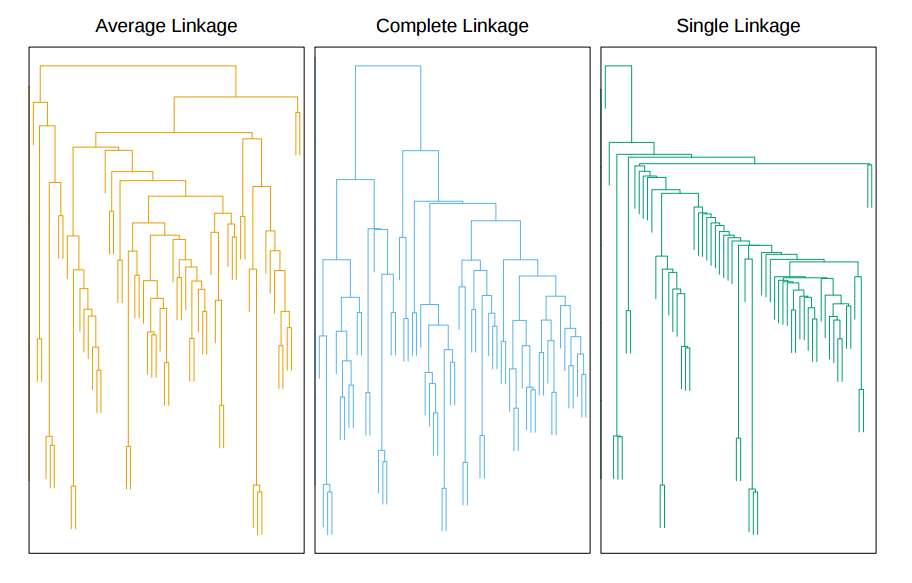
\includegraphics[width=\textwidth]{img/trees/dendrograms}
  \caption{Hierarchies over human tumor data produced by agglomerative clustering
    with three different linkage criterions. 
  Image from \citet{Hastie2009}.}
\label{fig:dendrograms}
\end{figure}

In divisive clustering, the approach is flipped.
We begin with a cluster containing
every data point, corresponding
to the root of the output tree.
We recursively
partition the cluster, until 
we are left with singleton clusters
at each leaf.
Partitioning a cluster
typically corresponds to solving
an optimization problem, such as minimizing
a cost function of a split.
For example, we could partition
a cluster using $k$-means, with $k = 2$,
optimizing the $k$-means cost function.
Alternatively in spectral clustering methods,
we create a similarity graph, $G$,
given a similarity function $s(\x, \x^\prime)$.
$G$ is an undirected, weighted graph
where there is a node for each data point,
and the weight for each edge $(i, j)$ is
$s(\x_i, \x_j)$ \citep{VonLuxburg2007}.
Bipartitioning a cluster
corresponds to finding a cut in its similarity graph,
and intuitively a good cut would avoid
edges between similar points.
Finding a good partition thus corresponds
to finding a minimum cut on $G$
for such cost functions as
RatioCut \citep{Hagen1992} and Ncut \citep{Shi2000}.

\iffalse
\subsection{Bayesian learning}
Bayesian learning is a probabilistic
approach to machine learning.
In Bayesian learning, our data
are represented as observed random variables,
which are generated conditionally
on a set of unobserved latent variables.
This is sometimes called a latent variable model.

In a latent variable model,
we have observed dataset $\dataset$
and assume there is some
unobserved set of latent variables $\globals$
responsible for generating $\dataset$.
The latent variables $\globals$
are distributed according
to a \emph{prior distribution} $\p(\globals)$,
and our observed data
are generated by a conditional
distribution $\p(\dataset \given \globals)$, also called
the \emph{likelihood}.
We are typically interested in the
\emph{posterior distribution},
$\p(\globals \given \data)$, which is the distribution
over latent variables given data.
Computing the posterior distribution is called \emph{inference}.
The posterior distribution can be calculated
via Bayes rule:

\begin{align}
  \p(\globals \given \dataset) = \frac{\p(\dataset \given \globals)\p(\globals)}{\p(\dataset)} = \frac{\p(\dataset \given \globals)\p(\globals)}{\int_\globals \p(\dataset \given \globals)\p(\globals)}
\end{align}

The choice of prior distribution and likelihood model
affect our ability to perform inference.
If our prior distribution is \emph{conjugate}
to our likelihood model, the posterior distribution
will be of the same form as the prior
and can be expressed analytically.
For example, if our prior over parameters
is Gaussian and likelihood model is Gaussian,
the posterior distribution will also be Gaussian.
This setup is common in classification problems
for real-valued data.
Similarly, if our prior over parameters is Dirichlet,
and the likelihood model is Multinomial,
the posterior distribution will be Dirichlet.
This setup is common in classification problems
when our data are bags-of-words.
In the general setting, however,
it is often impossible to compute an
analytical form for the posterior distribution.

After performing inference and obtaining
the posterior distribution $\p(\globals \given \dataset)$,
we are often tasked with prediction,
or calculating a distribution over a new, unobserved
data point. Let $\x^*$ be an unobserved test point.
The predictive distribution is defined
as $\p(\x^* \given \dataset)$, and can be obtained by
marginalizing the posterior distribution:

\begin{align}
  \p(\x^* \given \dataset) = \int_\globals \p(\x^*, \globals \given \dataset)d\globals =  \int_\globals \p(\x^* \given \globals, \dataset)\p(\globals \given \dataset)d\globals
\end{align}

%Statistical models are often represented
%as a directed graph, where nodes
%are random variables and edges
%represent dependency, called a \emph{graphical model}.

A classic example of a latent variable model
is the Gaussian mixture model (GMM).
GMM's are typically used in flat clustering scenarios,
and as such, we assume a fixed amount of clusters $K$.
A latent variable responsible for generating
data in a GMM are
the $K$ cluster centers, denoted by the set
$\bm{\mu} = \{\mu_1, \ldots, \mu_K\}$.
Each cluster has a weight, or a prior probability
of a data point belonging in the cluster,
represented by the vector $\bm{\pi} = \{\pi_1,\ldots,\pi_K\}$.
Each data point is generated by sampling a cluster
assignment $\z$ from the probability distribution $\bm{\pi}$,
and sampling a vector from a Gaussian distribution
centered at $\mu_\z$.
The graphical model for a GMM is pictured in \autoref{fig:gmm-model}.

\begin{figure}[H]
  \centering
  \includestandalone[width=0.2\textwidth]{tikz/gmm}
  \caption{A graphical model representation of a Gaussian mixture model. $\x_n$ is
  one of $\numdata$ data points and $\z_n$ is its cluster assignment. $\bm{\pi}$ are the weights
  for each cluster, and $\bm{\mu}$ are the centers of each cluster.}
\label{fig:gmm-model}
\end{figure}

Unfortunately, in the GMM,
and in many other latent variable models,
the posterior distribution $\p(\bm{\mu}, \bm{\pi} | X)$
is impossible to compute analytically.
Thankfully, there are plenty of
algorithms to approximate the posterior distribution,
such as
Markov chain
Monte Carlo (MCMC), or variational
inference.

Often times, we are not interested in the posterior
distribution itself, but the settings of the latent variables
that result in the highest posterior probability, i.e.
$\globals^* = \text{argmax}_\globals \p(\globals | X)$.
$\globals^*$ is called the \emph{maximum a posteriori}
and can be approximated 
by such algorithms as
expectation-maximization \citep{Dempster1977}.
\fi

\section{The generative process}

Bayesian nonparametric hierarchical clustering (BNHC)
is a latent variable model where
data is generated in
in two stages.
First, a tree is generated by a
\emph{tree prior}.
Conditioned on the sample
from the tree prior,
data is generated with
a \emph{tree likelihood model}.

The simplest tree priors
model \emph{cladograms},
or rooted binary trees
with data at the leaves,
but very often the trees are imbued with
additional information.
For example:

\begin{enumerate}
  \item An ordering on the internal nodes of the tree.
    Typically, the root is given the lowest number and
    each node will have a higher number than its parent.
  \item Times associated with each node.
    Nodes higher up in the tree will typically have
    earlier times, creating an evolutionary
    interpretation to the hierarchy.
\end{enumerate}

If we are only interested in tree structure,
not ordering or node times, we can simply discard
all auxiliary information at the very end.

\begin{figure}[H]
  \centering
  \includegraphics{tikz/lvm}
  \caption{The graphical model used
  in Bayesian hierarchical clustering. $\tree$
  is a tree, sampled from a tree prior distribution.}
  \label{fig:bhc-gen-model}
\end{figure}

Formally,
let $\tree$ be a class
of tree structures (e.g. ordered cladograms),
and let $\p(\tree \in \trees)$
be a tree prior
for $\trees$.
We sample parameters $\globals$ for tree likelihood model,
conditional on the tree structure.
This involves assigning
latent parameters to each internal node in the $\tree$
and specifying a stochastic process in which they are generated.
Conditioned on a particular
structure $\tree$ sampled from $\p(\tree)$
and tree likelihood parameters $\globals$, dataset
$\dataset$
is generated
via probability distribution $\p(\dataset \given \tree, \globals)$.
This is visualized as a graphical model in \autoref{fig:bhc-gen-model}
and concisely expressed as follows:

\begin{align*}
  \tree &\sim \p(\tree) \\
  \globals &\sim \p(\globals \given \tree) \\
  \dataset &\sim \p(\dataset \given \tree, \globals)
\end{align*}

Inference involves computing the posterior
distribution over trees and parameters, 
$\p(\tree, \globals \given \dataset)$, but we are sometimes interested
in the
posterior marginal distribution $\p(\tree \given \dataset)$.
Both of these distributions are typically
impossible to compute
analytically as marginalizing over $\tree$
is intractable.
In practice, most methods use Markov chain Monte Carlo
methods to sample $\p(\tree, \globals \given \dataset)$
and $\p(\tree \given \dataset)$.

In this section, we will cover two broad
classes of tree priors and touch on
some extraneous models. We will then explain
a few tree likelihood models, and 
finish by explaining how to perform
inference in Bayesian hierarchical clustering.

\subsection{Tree priors}

Broadly speaking, 
tree priors can be broadly broken down into 
\emph{coalescent} models
and 
\emph{diffusion} models.
Both of them share a core characteristic
of being sequential models.
In coalescent models, the tree is built sequentially
from the bottom up. We begin with each
data point in its own cluster,
and sequentially merge clusters until
there is only one. This idea is
very similar to agglomerative clustering.
Diffusion models take an inductive approach,
where we begin with a hierarchy over a single
data point, and sequentially add data to the hierarchy until
we have a tree with $\numdata$ leaves,
a fundamentally different paradigm.
Shared in both types of models is the property
of
\emph{exchangeability}.
A sequence of random variables, $\x_1, \ldots, \x_\numdata$,
is considered exchangeable
if their joint distribution
is invariant to permutations of the variables.
Exchangeability often enables computationally efficient
inference algorithms.

\subsubsection*{Coalescent models}

Coalescent modeling was developed
in the early 1980s by John Kingman,
and achieved success in the field
of population genetics
\citep{Kingman1982}.
Coalescent models assume a
continuous time process,
where in individuals of a population
are traced backwards in time
through their ancestry until
they all share a single common ancestor.
In terms of hierarchical clustering,
the individuals in the population
correspond to a dataset $\dataset$,
and their
ancestry backwards in time
is a hierarchy.

The classic coalescent model is
Kingman's coalescent \citep{Kingman1982}.
It assumes a countably infinite population
but has a consistency property
which allows it to be described
in terms of its marginal distribution
over finite populations.

Consider a dataset $\dataset$ with $\numdata$ points, 
which we will call ``individuals''.
In Kingman's coalescent,
our current population exists at time $t = 0$,
and each individual in the population has a single
parent in the previous generation, which has its own parent,
continuing backwards in time until
$t = -\infty$. 
At some time in the past,
the lineage of any two individuals will ``coalesce''
when they share an ancestor.
The lineages of the members of the population
can be concisely described
by the
\emph{genealogy} function, $\pi(t)$,
that maps between time $t$
and a partition of $\{1, \ldots, \numdata\}$
that groups individuals together
if their lineages have coalesced at time $t$.
$\pi(0) = \{\{1\}, \{2\},\ldots,\{\numdata\}\}$
represents
the current time, when no
lineages have coalesced.
$\pi(-\infty) = \{\{1, 2, \ldots, \numdata\}\}$
is the partition of all
individuals into a single group,
when they all share a common ancestor \citep{Teh2008}.

Kingman's coalescent
is a probability distribution
over genealogy functions $\pi(t)$
for populations of size $\infty$,
and the marginal distribution for
populations of size $\numdata$ is called the $\numdata$-coalescent.
The $\numdata$-coalescent
is a continuous-time
Markov process
over the space of partitions
of size $\numdata$,
starting at time $t = 0$ with
$\pi(0) = \{\{1\}, \{2\},\ldots,\{N\}\}$,
going backwards until  $t = -\infty$,
with
$\pi(-\infty) = \{\{1, 2, \ldots, N\}\}$.

\begin{figure}[H]
  \centering
  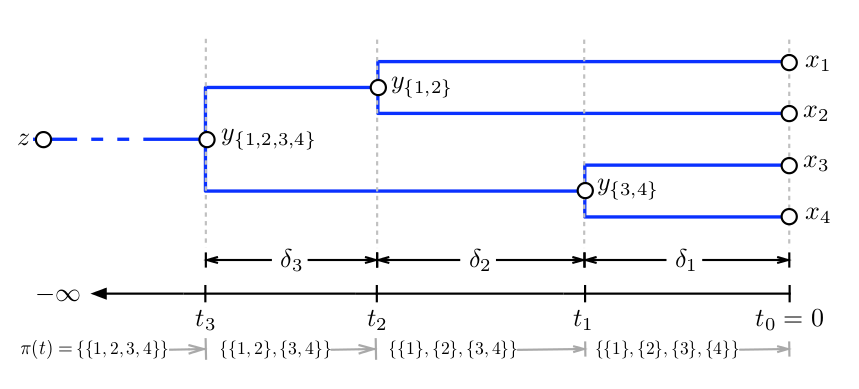
\includegraphics[width=\textwidth]{img/trees/coalescent}
  \caption{A sample from Kingman's coalescent. $\z$ is
  the common ancestor for data $\x_1, \x_2, \x_3, \x_4$. Each $y_C$
  represents the common ancestor for data subset $C$. 
  The axis represents time, and each $\delta_i$ represents elapsed time between
  coalesce events. Finally, $\pi(t)$ is
  the genealogy function. Image taken from \citet{Teh2008}.}
\label{fig:coalescent}
\end{figure}

The $\numdata$-coalescent
can be broken down into two
independent components.
The first is the \emph{jump process},
which models the discrete transitions
between partitions
before and after coalesce events.
The second is the \emph{time process},
which models the times in the past
at which coalesce events happen.
The jump process is very simple.
Each lineage has an equal probability of merging
with any other lineage. Thus, the
jump process is a Markov chain
where the transition matrix is uniform
for each pair in a partition coalescing.
The jump process has $\numdata - 1$ transitions, starting
with the partition with singleton groups
for each data, and ending with the
partition with all data in a single group.
The time process produces a series of times
$t_{\numdata - 1} < t_{\numdata - 2} < \cdots <  t_1$ when coalesce events happen,
ending with $t_0 = 0$.
The first step in the jump process
corresponds to coalesce time $t_1$, and so on.
Kingman's coalescent assumes
that each pair of lineages merges at a constant rate of $1$,
i.e.\
a pair lineages will eventually merge at
$t \sim \text{Exp}(1)$ where $\text{Exp}$ is the exponential distribution.
Given a set of $m$ lineages,
a pair of them will merge at
$t \sim \text{Exp}(\binom{m}{2})$.
Let the elapsed time before each jump $i$ be
$\delta_i = t_{i - 1} - t_i$
We start with a population of size $\numdata$,
and it decreases by $1$
in each step of the jump process.
Thus, $\delta_i \sim \text{Exp}(\binom{\numdata - i + 1}{2})$.
After sampling all the $\delta_i$'s, we can easily
compute the coalesce times,
completing the distribution over genealogy functions.
An example sample from Kingman's coalescent can be
seen in \autoref{fig:coalescent}.

\begin{figure}[H]
  \centering
  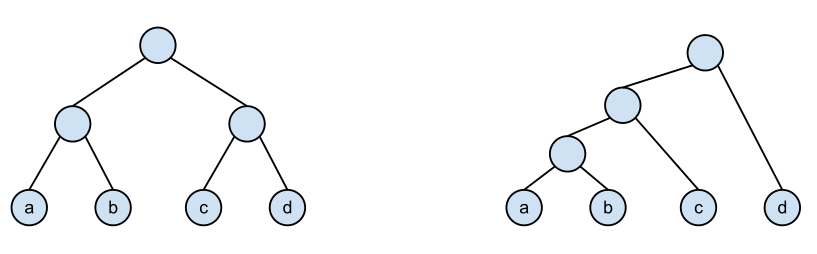
\includegraphics[width=0.5\textwidth]{img/trees/balanced}
  \caption{For the balanced tree on the left, there are two
  possible orderings in which clusters were merged, whereas there is only one possible ordering for the unbalanced tree on the right. Image taken from \citet{Boyles2012}.}
\label{fig:balanced}
\end{figure}

A genealogy sampled from Kingman's coalescent
is an ordered cladogram with times associated with every internal node.
The ordering comes from the order in which
internal nodes were created in the jump process.
The induced distribution over just ordered trees
is in fact uniform \citep{Teh2008}.
However, we often don't need order information
in hierarchical clustering.
\citet{Boyles2012} computes the induced distribution over
unordered rooted binary trees.
For a given unordered tree with $\numdata$ leaves, $\tree$,
there are $\frac{(\numdata - 1)!}{\prod_{\n = 1}^{\numdata - 1}m_\n}$ possible orderings
where $m_\n$ is the number of internal nodes in the subtree
of $\tree$ indexed by $\n$. 
Intuitively, there
are several possible orderings to create a perfectly balanced binary tree,
but only one for an extremely unbalanced binary tree (see \autoref{fig:balanced}).
Thus, Kingman's coalescent induces a prior distribution
over unordered trees
that favors balanced trees over unbalanced trees,
and 
marginalizing out the ordering of internal
nodes results in this distribution, also called
the time-marginalized coalescent \citep[TMC; ][]{Boyles2012}.

Kingman's coalescent assumes constant merge rates
for each pair of lineages in a genealogy. 
Although this is an intuitive assumption,
there have been several papers generalizing Kingman's coalescent
to both $k$-ary trees, and more complex coalesce rates.
For example, in \citet{Pitman1999}, Pitman introduced the
$\Lambda$-coalescent, extending Kingman's coalescent
to have ``multiple collisions'', supporting
$k$-ary trees.
Rather than the coalesce rate
being $1$, it is instead $\lambda_i^k$
where $k$ is the maximum number of lineages
that can merge in a single event and $i$ is the total number
of lineages at the time of the event, resulting in $\delta_i \sim \text{Exp}(\lambda_i^k)$. $\lambda_i^k$ is calculated as
\begin{align}
  \lambda_i^k = \int_0^1 \gamma^{k - 2}(1 - \gamma)^{(i-k)}\Lambda(d\gamma)
\end{align}
where $\Lambda$ is a finite measure on $[0, 1]$. The
$\Lambda$-coalescent is identical to Kingman's coalescent
when $k = 2$ and $\Lambda$ is the Dirac delta.
Setting $\Lambda$ to a beta measure
results in the aptly named beta-coalescent \citep{Hu2013}.
A description of such coalescent rate functions
can be seen in \citet{Aldous1999}.

\subsubsection*{Diffusion models}
Diffusion models adopt a different paradigm for generation.
In diffusion models, we begin with a
trivial tree over just one data point. We then
grow the tree by iteratively attaching new data
to branches in the tree, eventually creating
a tree with $\numdata$ leaves.
Similar to coalescent models, there is an underlying
continuous time process responsible for
the tree structure.

The first diffusion model, the Dirichlet diffusion tree (DDT),
was proposed by Radford Neal in 2003 \citep{Neal2003}.
The DDT is an exchangeable model that models a sequence of data
$\x_1, \x_2,\ldots,\x_N$.
There is an underlying continuous time process
that lasts from time $t = 0$ to $t = 1$
In essence, each data point is generated in sequence by
a random walk beginning at $t = 0$,
reaching a final value at $t = 1$.
Each data point initially follows the previous
random walks, but eventually diverges and continues independently.

Let $\x_\n(t)$ be the value of data point $\x_\n$
at time $t$, defining a ``path'' associated
with each point from its start $\x_\n(0)$ to its final (observed) value $\x_\n(1)$.
In addition, the path of each data point $\x_\n(t)$ is conditioned
on all previous paths $\x_1(t), \x_2(t), \ldots, \x_{\n - 1}(t)$.
This process, when completed for all $\numdata$ data points,
induces a binary tree over the data.

The path for the first data point $\x_1$
is a Brownian motion
beginning at the origin.

\begin{align}
  \x_1(0) &= 0 \\
  \x_1(t + dt) &= \x_1(t) + \N(0, \sigma^2Idt)
\end{align}

The path for the second data point $\x_2(t)$
is exactly $\x_1(t)$ until
at some time $\tree$ it diverges,
creating a branching point for
$\x_1(t)$ and $\x_2(t)$.
$\tree$ is sampled according to an \emph{acquisition function}
$a(t)$ and
after divergence, $\x_2(t)$ is an
independent Brownian motion.

Now consider the inductive case.
We have already sampled $\n - 1$
paths, which form a binary tree
with internal nodes corresponding to
divergence events.
$\x_n(t)$ initially follows the same
path as the previous points.
If $\x_1(t)$ is traversing a path
followed by $m$ previous paths,
the probability that $\x_1(t)$ will
diverge along an infinitesimally small
interval $d$ is 
$a(t)dt/m$. 
In practice we work with the cumulative
divergence function $A(t) = \int_0^t a(u)du$.
Given an interval of time $(s, t)$,
that lies on a single branch of the DDT
that was previously traversed by $m$ paths,
the probability that the next point
does not diverge on the interval
is $e^{(A(s) - A(t))/m}$.
The acquisition function is chosen such that
$a(1) = \infty$. This guarantees that
all data points must diverge 
before $t = 1$. 
For a visualization of a DDT
for 1-dimensional data, see \autoref{fig:ddt-vis}.
Possible choices of acquisition function
are $a(t) = \frac{c}{1 - t}$ or $a(t) = b + \frac{d}{1 - t^2}$,
where $b$, $c$, and $d$ are constants.

\begin{figure}[H]
    \centering
    \begin{subfigure}[b]{0.45\textwidth}
        \centering
        \includegraphics[width=\textwidth]{img/trees/ddt}
    \end{subfigure}
    \hfill
    \begin{subfigure}[b]{0.45\textwidth}
        \centering
        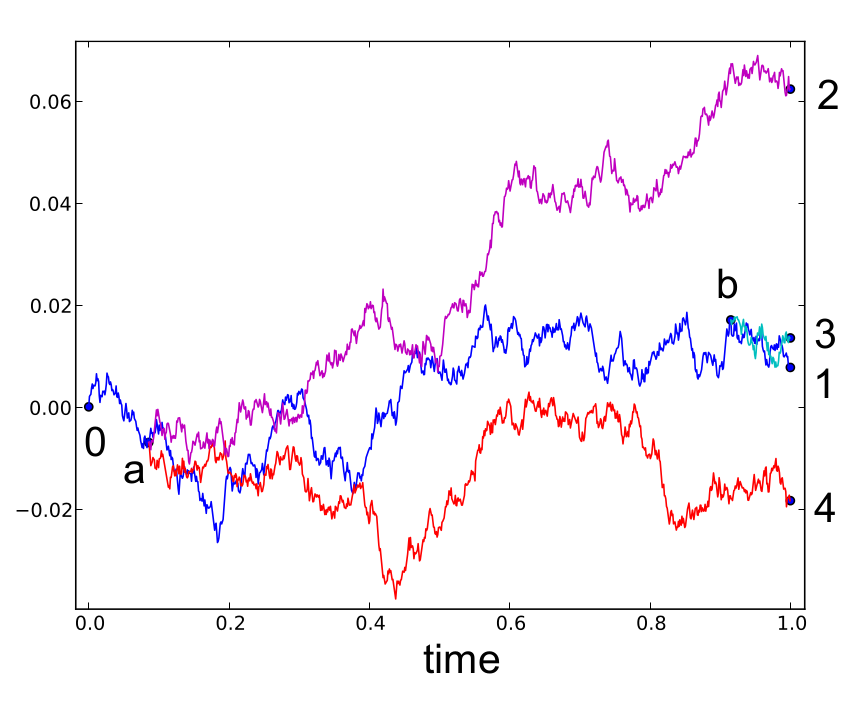
\includegraphics[width=\textwidth]{img/trees/pydt}
    \end{subfigure}
    \caption{
      On the left is a sample from a Dirichlet diffusion tree with 4 points.
      Black dots correspond to nodes in the tree. The image is taken from \citet{Vikram2016}.
      On the right is a sample from a Pitman-Yor diffusion tree with 4 points.
      Black dots correspond to nodes in the tree. Notice
      that the first internal node has a branching factor of 4,
      whereas the rest have a branching factor of 2.
      The image is taken from \citet{Knowles2015}.
    }
    \label{fig:ddt-vis}
\end{figure}

The DDT, as proposed in \citet{Neal2003}, 
jointly models the tree prior and tree likelihood model.
However, we can consider the same
path reinforcement model, without the Brownian motion
to obtain a prior over ordered cladograms
with times for each node.
We can obtain a sample from the DDT and just ignore the
internal values at each node where divergence occurred.

The DDT thus induces a prior over ordered cladograms
with times.
Unlike Kingman's coalescent, however, the DDT
does not, in general, induce a uniform prior over ordered cladograms.
This is due to the path-reinforcement element
of the prior and the choice of acquisition function.
It is worth noting that the Dirichlet diffusion tree has achieved
great success in the area of density estimation \citep{Adams2008}.

An extension to the Dirichlet diffusion tree
is the Pitman-Yor diffusion tree (PYDT),
which removes the DDT's restriction to just binary trees
\citep{Knowles2015}.
In a Pitman-Yor diffusion tree, the probability
of a data point diverging in an infinitesimally small
interval $dt$ is
\begin{align}
  \frac{a(t)\Gamma(m - \beta)}{\Gamma(m + 1 + \alpha)}
\end{align}
where $\alpha$ and $\beta$ are parameters. Setting $\alpha = \beta = 0$,
results in same probability as in the DDT.
In the PYDT, a data point can not only
diverge at any point in time,
but can also diverge at a branching point
in the tree, where in the DDT
a data point would always pick a branch.
When a data point reaches a branching point,
it picks branch $k$
with probability
\begin{align}
  \frac{b_k - \beta}{m + \alpha}
\end{align}
where $b_k$ is the number of paths
that previously traversed $k$
and $m$ is total the number of paths
that reached the branching point.
The probability that the data point
diverges, creating a new branch, is
\begin{align}
  \frac{\alpha + \beta K}{m + \alpha}
\end{align}
where $K$ is current number of branches.
This scheme allows for an arbitrary amount of
branching at each internal node of the tree,
but can be tuned by settings of $\alpha$ and $\beta$.
Note again that when $\alpha = \beta = 0$,
the generation scheme matches the DDT.

\subsection{Generalizations of coalescent and diffusion models}

The simplest distribution over (unordered) cladograms
is the uniform.
Kingman's coalescent is one step away,
as it
induces the uniform distribution
over ordered cladograms,
a distribution also called
the Yule model \citep{Harding1971}.
Marginalizing over possible orderings
results in the TMC \citep{Boyles2012}, a distribution over unordered cladograms biased towards balanced trees.

Generalizations of Kingman's coalescent
include the $\Lambda$-coalescent \citep{Pitman1999},
which extends coalescents to multifurcating trees,
and the Aldous $\beta$-splitting model \citep{Aldous1996}.
A more recent model, the Gibbs fragmentation tree,
is a generalization of the $\beta$-splitting model
to multifurcating trees,
and is considered the most general Markovian distribution over trees \citep{McCullagh2008}.

The diffusion models on the other hand,
include far more parameters.
The choice of acquisition function,
along with the choice of $\alpha$ and $\beta$ in the PYDT,
result in a wider variety of distributions.
The PYDT's induced distribution over tree
structure is, in fact, a specific case
of the Gibbs fragmentation tree.

An alternate generalization is the fragmentation-coagulation process (FCP),
which is a distribution over partition-valued
Markov chains \citep{Teh2011}.
Instead of partitions being
split up or merged monotonically as in
diffusion and coalescent models, the 
FCP models both split and merge
transitions in the Markov chain, encompassing
both coalescent and diffusion models.

All of these relationships are pictured in \autoref{fig:familytree}.

\begin{figure}[H]
  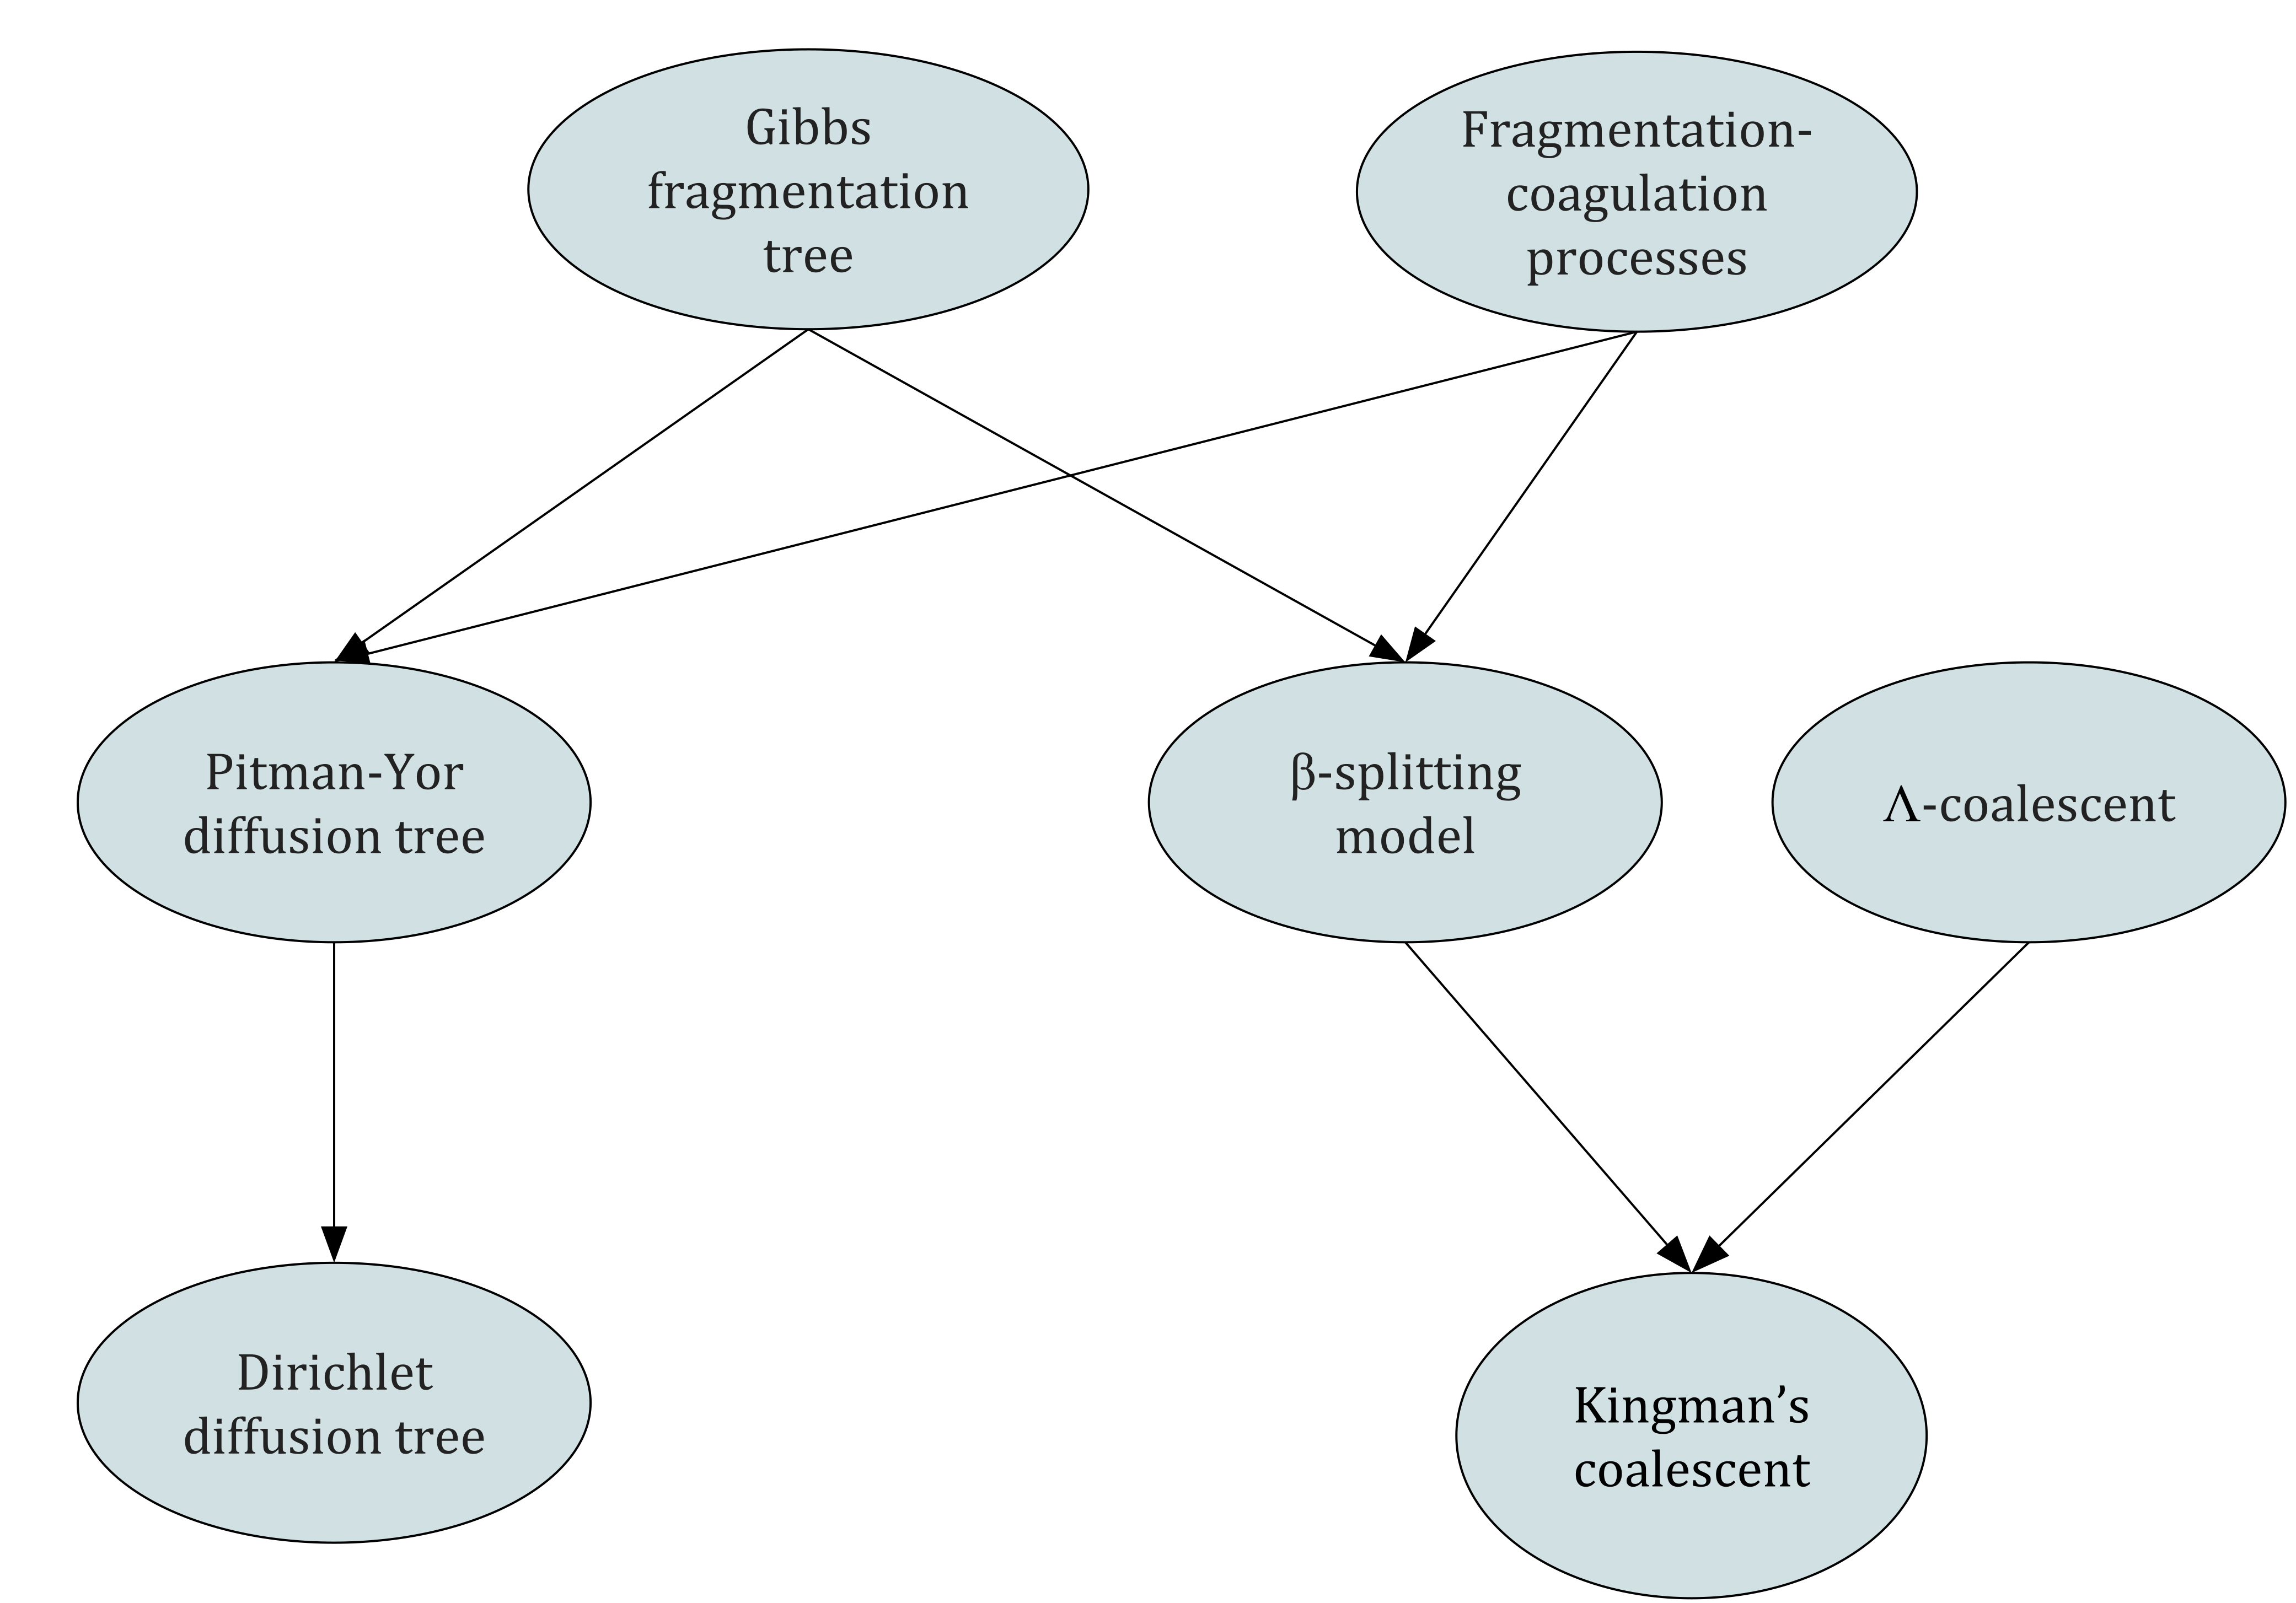
\includegraphics[width=\textwidth]{img/trees/FamilyTree}
  \caption{A graph visualization of the relationships between various
  tree priors. Directed arrows represent
  specific cases of a distribution or model.}
\label{fig:familytree}
\end{figure}

\subsection{Other priors}

A popular line of work
follows extensions of the Chinese restaurant
process (CRP) and other related Bayesian nonparametric objects.
The CRP is a distribution
over partitions of $\{1, \ldots, N\}$ \citep{Aldous1985}.
Its name derives
from the nature of the stochastic process
by which partitions are sampled.
Imagine an empty restaurant with
a countably infinite number of tables
labeled $1, 2, \ldots$
with a line of customers waited to be seated.
The first customer will always pick 
table $1$.
Let $\alpha$ be a hyperparameter.
The $n + 1$-th customer will pick the
the $i$-th table with probability
\begin{align}
    \frac{c_i}{n + \alpha}
\end{align}
where $c_i$ is the number
of customers already sitting at
table $i$ or
sit at a new, unoccupied table with probability
\begin{align}
    \frac{\alpha}{n + \alpha}
\end{align}
After $\numdata$ customers have been seated,
we have a partition over $\{1,\ldots, N\}$,
where customers are grouped
by the table they are seated at.

\begin{figure}[t]
  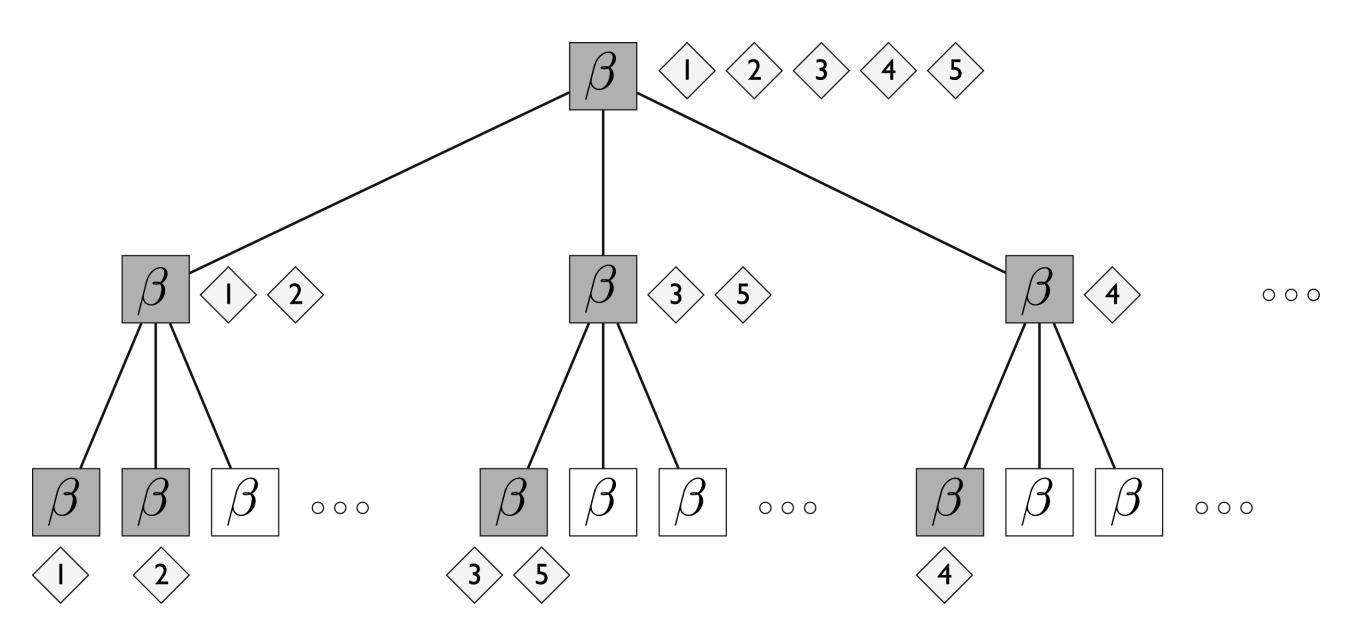
\includegraphics[width=\textwidth]{img/trees/ncrp}
  \caption{A visualization of a sampled from
  a nested Chinese
  restaurant process (NCRP). Only three levels
  for 5 customers are shown.
  Image from \citet{Blei2010}.}
\label{fig:ncrp}
\end{figure}

The CRP is an exchangeable model
and has a reinforcement property, where
tables with more people attract 
even more people. It is
also the basis of the nested Chinese
Restaurant Process (nCRP) model
used for hierarchical clustering \citep{Blei2010}.
The nCRP extends the analogy to
an infinite chain of restaurants.
After a customer goes and sits
at the first Chinese restaurant,
they are directed to yet another
Chinese restaurant where the process
repeats ad infinitum. This defines
a structure where $\numdata$ customers, or data,
are distributed
across infinitely deep leaves of a tree.
Although the tree is infinite,
it can be represented in terms of its
finite induced distribution over
how the partition of customers is split
at each level of the tree. 
This results in a distribution over rooted trees
with arbitrary branching factor and ordering over internal nodes.
See \autoref{fig:ncrp} for a visualization of the NCRP.
The NCRP
is closely related to the nested Dirichlet process (NDP),
the underlying de Finetti measure for the NCRP.
An extension
of the NCRP and NDP is the nested hierarchical Dirichlet
process (NHDP) \citep{Paisley2014}. Whereas each datum in the NDP and NCRP
are each represented as an infinitely deep path
down the tree, each datum in the NHDP
is represented as a \emph{mixture} of
infinitely deep paths down the tree. 
The NCRP, NDP, and NHDP have been used to success
in topic modeling, finding hierarchies over
a corpus of documents.

The tree-structured stick-breaking process (TSSB)
is an alternate model 
where data are allowed to live at any node
in the tree, as opposed to just leaves \citep{Adams2010}.
At the core of the TSSB is the
stick-breaking process, a Bayesian nonparametric object
closely related to the CRP.
The stick breaking process
iteratively carves up the unit interval
into smaller and smaller pieces,
resulting in an infinite amount of ``sticks'',
whose lengths sum up to one.
Let $\beta_i \sim \text{Beta}(1, \alpha)$ for
$i \in 1,2,\ldots$.
These will be fractions of the remainder
of the stick that we will carve up.
Now, let the ``sticks''
be $t_1 = \beta_1$ and $t_i = \beta_i \prod_{j = 1}^i (1 - \beta_j)$.
We now have a sequence of
random variables, $t_1, t_2, \ldots$
such that $\sum_{i = 1}^\infty t_i = 1$,
which we can treat as a distribution over
an infinite amount of events.
The TSSB is an extension of the stick-breaking process
to generate a distribution
over infinitely deep and wide hierarchies.
Associated with each internal node in the tree
is a stick breaking process,
which acts as a distribution over an infinite
amount of branches out of the node.
Data are generated by starting at the root
and sampling a branch. At any point,
data have a probability of stopping at a given node,
which distributed as a stick breaking process
over each possible path heading down the tree.
Although the tree is infinite, it induces a distribution
over trees where $\numdata$ data live across every node
in the tree, a fundamentally different tree structure
from the previous ones.

\subsection{Tree likelihood models}

Given a sample from a tree structure prior, 
we now need a scheme to sample
hierarchically structured data.
Let the sample from the tree
structure prior be $\tree$.
Assume, for now, $\tree$ is
an rooted tree,
with times associated with each internal node (ordering does not matter).
The standard tree likelihood model is a diffusion model,
where there is a parameter $\globals_\n$ for each internal
node $\n$, which are generated from the root downwards.
Let $\globals_0$ be the parameter associated with the root node,
which will be sampled according to a prior distribution $\p_0(\globals)$.
We then define a transition kernel, $T(\globals' \given \globals)$.
The parameter for each node is generated conditionally
given its parent parameter in the tree,
i.e. for node $v$ and its parent $u$,
$\globals_v \sim T(\cdot \given \globals_u)$.
Data at leaves are also generated in this fashion.
We now enumerate some transition kernels
which accomodate different data types and tree structures.

\begin{enumerate}
    \item \textbf{Generalized Gaussian diffusion.} If our data
    is continuous and $\d$-dimensional, we can associate
    a latent vector $\globals_\n \in \R^\d$ with each internal node
    $\n$ in the tree. Let $u$ be an internal node
    and $v$ one of its children and
    let $\delta_{uv}$ be the elapsed time between $u$ and $v$.
    We sample $\globals_v \sim \N(\globals_u, \Sigma\delta_{uv})$,
    where $\Sigma$ is a positive definite covariance matrix.
    The root node value is assigned a prior
    $\N(\mu_0, \Sigma_0)$.
    In the case where there are no times associated with each node,
    we can assume elapsed time between nodes is always 1,
    and the hyperparameters in the model would be
    $\Sigma$, $\mu_0$, and $\Sigma_0$.
    This approach is used in \citet{Neal2003}, \citet{Teh2008}, \citet{Knowles2015},
    \citet{Adams2010}, \citet{Boyles2012} and \citet{Hu2013}.
    \item \textbf{Multinomial diffusion.} If our data
    consists of several categorical variables, 
    we can model it with a transition matrix, $\tree$.
    For categorical feature $c$, let $T_c$ 
    be the row in $\tree$ for feature $c$.
    Let $\delta_{uv}$ be the elapsed time between parent $u$ and child $v$.
    As suggested by
    \citet{Teh2008},
    $T_{c} = e^{-\lambda_{c}\delta_{uv}}I + (1 -  e^{-\lambda_{c}\delta_{uv}})q_{c}^T\bm{1}$
    where $\lambda_{c}$ is a hyperparameter for the evolution rate for feature 
    $c$, $q_{c}$ is a hyperparameter for the equilibrium
    distribution of $c$, and $\bm{1}$ is a vector of ones.
    \item \textbf{Dirichlet-Multinomial diffusion.}
    This tree likelihood model is for
    trees without times associated with each internal node.
    When data consists of counts of discrete events,
    such as the bag of words in topic modeling,
    leaves can be described as sampling
    a multinomial distribution.
    The transition kernel for
    just internal nodes as suggested by \citet{Adams2010} is $T(\globals' | \globals) = \text{Dirichlet}(\kappa\globals)$
    and the prior is $P_1(\globals) = \text{Dirichlet}(\kappa\bm{1})$,
    where $\kappa$ is a concentration hyperparameter and $\bm{1}$ is a
    vector of ones.
    Leaves are sampled via a multinomial distribution
    with its parent's vector as its parameter.
\end{enumerate}

\subsection{Inference}

We are interested
in the posterior distribution
over hierarchies given data.
Typically, this distribution
is intractable to compute
analytically, so approximate
methods are required.
A popular approach used
in \citet{Neal2003}, \citet{Knowles2015}, and \citet{Boyles2012}
is the Metropolis-Hastings
algorithm,
a Markov chain Monte Carlo
method where samples
are used as an approximation
to the posterior distribution.

In Metropolis-Hastings,
we are given a target
distribution, $\p(\x)$, and
define a \emph{proposal distribution}, $\q(\x^\prime \given \x)$.
A Markov chain is initialized with state $\x_0$.
In each iteration of the algorithm
we use current state $\x_t$
to sample a candidate $\x^\prime$ from $\q(\x^\prime \given \x_t)$.
and then calculate
the acceptance ratio, 
\begin{align}
    \alpha = \frac{\p(\x^\prime)\q(\x_t \given \x^\prime)}{\p(\x_t)\q(\x^\prime \given \x_t)}
\end{align}
If $\alpha \ge 1$, we accept,
setting $\x_{t + 1} = \x^\prime$.
If $\alpha < 1$, we accept
with probability $\alpha$, and reject
otherwise, setting $\x_{t + 1} = \x_t$.
Provided some conditions on $\q(\x^\prime \given \x)$,
the Markov chain's stationary distribution
will be $\p(\x)$.

In BNHC, the probability distribution
of interest
is the posterior distribution $\p(\tree, \globals \given \dataset)$.
The state of a Markov chain in Metropolis-Hastings is therefore
a tuple $(\tree, \globals)$.
A proposal distribution $\q(\tree^\prime, \globals^\prime \given \tree, \globals, \dataset)$ would need to jointly
sample $\tree$ and $\globals$.
A simple strategy is to have two proposal distributions: a 
tree proposal $\q(\tree^\prime \given \tree)$
and parameter proposal $\q(\globals^\prime \given \tree^\prime, \globals)$. 
We would sample $\tree^\prime$ first,
and then we would sample $\globals^\prime$ 
additionally conditioned on $\tree^\prime$.
Alternatively, if we're only interested
the posterior distribution over trees,
we can often marginalize out $\globals$, either
analytically or via belief propagation,
resulting in the posterior marginal
distribution $\p(\tree \given \dataset)$.

\begin{figure}[t]
  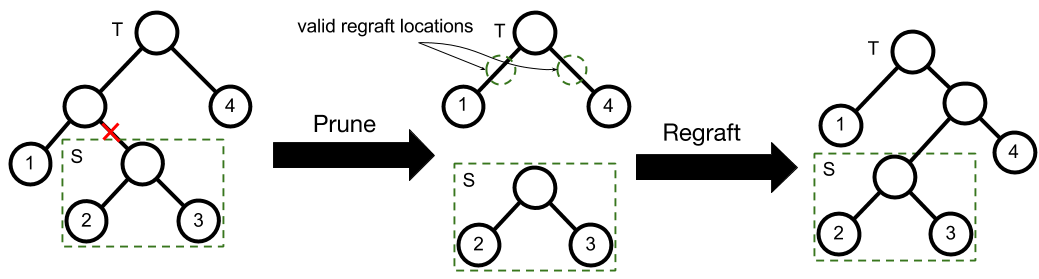
\includegraphics[width=\textwidth]{img/trees/spr}
  \caption{Visualization of a subtree-prune and regraft move for a
  tree with four leaves. Image from \citet{Vikram2016}.}
\label{fig:spr}
\end{figure}

Designing a tree proposal distribution
involves modifying some tree $\tree$ 
randomly to form a new tree $\tree^\prime$.
One of the most popular proposals
is the \emph{subtree-prune and regraft} (SPR) move, proposed by \citet{Swofford1990}.
An SPR move consists of a \emph{prune} followed by a \emph{regraft}.
Let $\tree$ be a tree.
Let $s$ be a non-root
node in $\tree$ selected uniformly at random
and $S$ be its corresponding subtree.
We first \emph{prune}
$S$ from $\tree$ by
remove $s$'s parent $p$ from the tree,
replacing $p$ with $s$'s sibling.
To regraft $p$ to $\tree$,
we first select a branch in $\tree$,
$(u, v$), where $u$ is the parent of $v$.
$S$ is re-attached to $\tree$
by creating a new node $p$
with parent $u$ and children $v$ and $s$,
creating a new tree $\tree^\prime$.
This process is visualized in \autoref{fig:spr}.

The branch selected in the regraft move
is often sampled from a distribution
related to the tree prior.
For example, if we used a DDT,
we have a posterior distribution
over branches where a new data point would 
diverge. If such a distribution
does not exist, the branch can simply
be selected uniformly at random.

Two alternatives to the SPR move
moves are the leaf move,
which restricts the SPR move
to just leaf nodes,
and nearest-neighbor interchange
moves, which interchange
two pairs of subtrees.
It is worth noting
that 
the worst case mixing rate of
a Markov chain using
leaf moves to sample
the uniform distribution over
$\numdata$-leaf cladograms is $O(\numdata^3)$ \citet{Aldous2000}.

Sampling the parameters of 
the tree likelihood model is much simpler
than sampling the tree prior.
The parameters $\globals$ often
have conditional dependence
structure that allows simple
ancestral sampling or Gibbs sampling.
For example, in the DDT and Kingman's coalescent,
each internal node in the tree stores
a latent vector, representing the intermediate value
of data higher up in the tree.
If the likelihood model is
generalized Gaussian diffusion,
all conditional distributions are Gaussian.
We can thus Gibbs sample each of the
latent vectors.

Metropolis-Hastings is perhaps the
simplest method to sample a general
BNHC model. However, alternative methods
have been proposed,
such as using slice sampling in \citet{Adams2010},
sequential Monte Carlo in \citet{Teh2008} and \citet{Hu2013},
Gibbs sampling in \citet{Blei2010},
and variational inference in \citet{Paisley2014}.
Furthermore, there are greedy algorithms
to approximate a MAP estimate
to the posterior distribution
of trees given data \citep{Teh2008, Hu2013}.
